%
% $RCSfile: standards.tex,v $
%
% Copyright (C) 2002-2008. Christian Heller.
%
% Permission is granted to copy, distribute and/or modify this document
% under the terms of the GNU Free Documentation License, Version 1.1 or
% any later version published by the Free Software Foundation; with no
% Invariant Sections, with no Front-Cover Texts and with no Back-Cover
% Texts. A copy of the license is included in the section entitled
% "GNU Free Documentation License".
%
% http://www.cybop.net
% - Cybernetics Oriented Programming -
%
% http://www.resmedicinae.org
% - Information in Medicine -
%
% Version: $Revision: 1.1 $ $Date: 2008-08-19 20:41:09 $ $Author: christian $
% Authors: Christian Heller <christian.heller@tuxtax.de>
%

\section{Standards}
\label{standards_heading}
\index{Medical Informatics Standards}

In a further thought, current standards of medical informatics had to be
considered for the development of \emph{Res Medicinae} application modules.
There exists a whole plethora of (partly \emph{de facto}) standards -- far too
many to discuss here. The following sections will give a brief overview of only
a few standards which are potentially important for EHR development.

%
% $RCSfile: overview.tex,v $
%
% Copyright (C) 2002-2008. Christian Heller.
%
% Permission is granted to copy, distribute and/or modify this document
% under the terms of the GNU Free Documentation License, Version 1.1 or
% any later version published by the Free Software Foundation; with no
% Invariant Sections, with no Front-Cover Texts and with no Back-Cover
% Texts. A copy of the license is included in the section entitled
% "GNU Free Documentation License".
%
% http://www.cybop.net
% - Cybernetics Oriented Programming -
%
% http://www.resmedicinae.org
% - Information in Medicine -
%
% Version: $Revision: 1.1 $ $Date: 2008-08-19 20:41:08 $ $Author: christian $
% Authors: Christian Heller <christian.heller@tuxtax.de>
%

\subsection{Overview}
\label{overview_heading}
\index{Medical Informatics Working Groups}
\index{Deutsches Institut fuer Normung}
\index{DIN}
\index{Comite Europeen de Normalisation}
\index{CEN}
\index{International Organization for Standardization}
\index{ISO}

Figure \ref{groups_figure} shows the medical informatics working groups of
important standardisation organisations, namely the:

\begin{itemize}
    \item[-] \emph{Deutsches Institut fuer Normung} (DIN)
    \item[-] \emph{Comite Europeen de Normalisation} (CEN)
    \item[-] \emph{International Organization for Standardization} (ISO)
\end{itemize}

\begin{figure}[ht]
    \begin{center}
        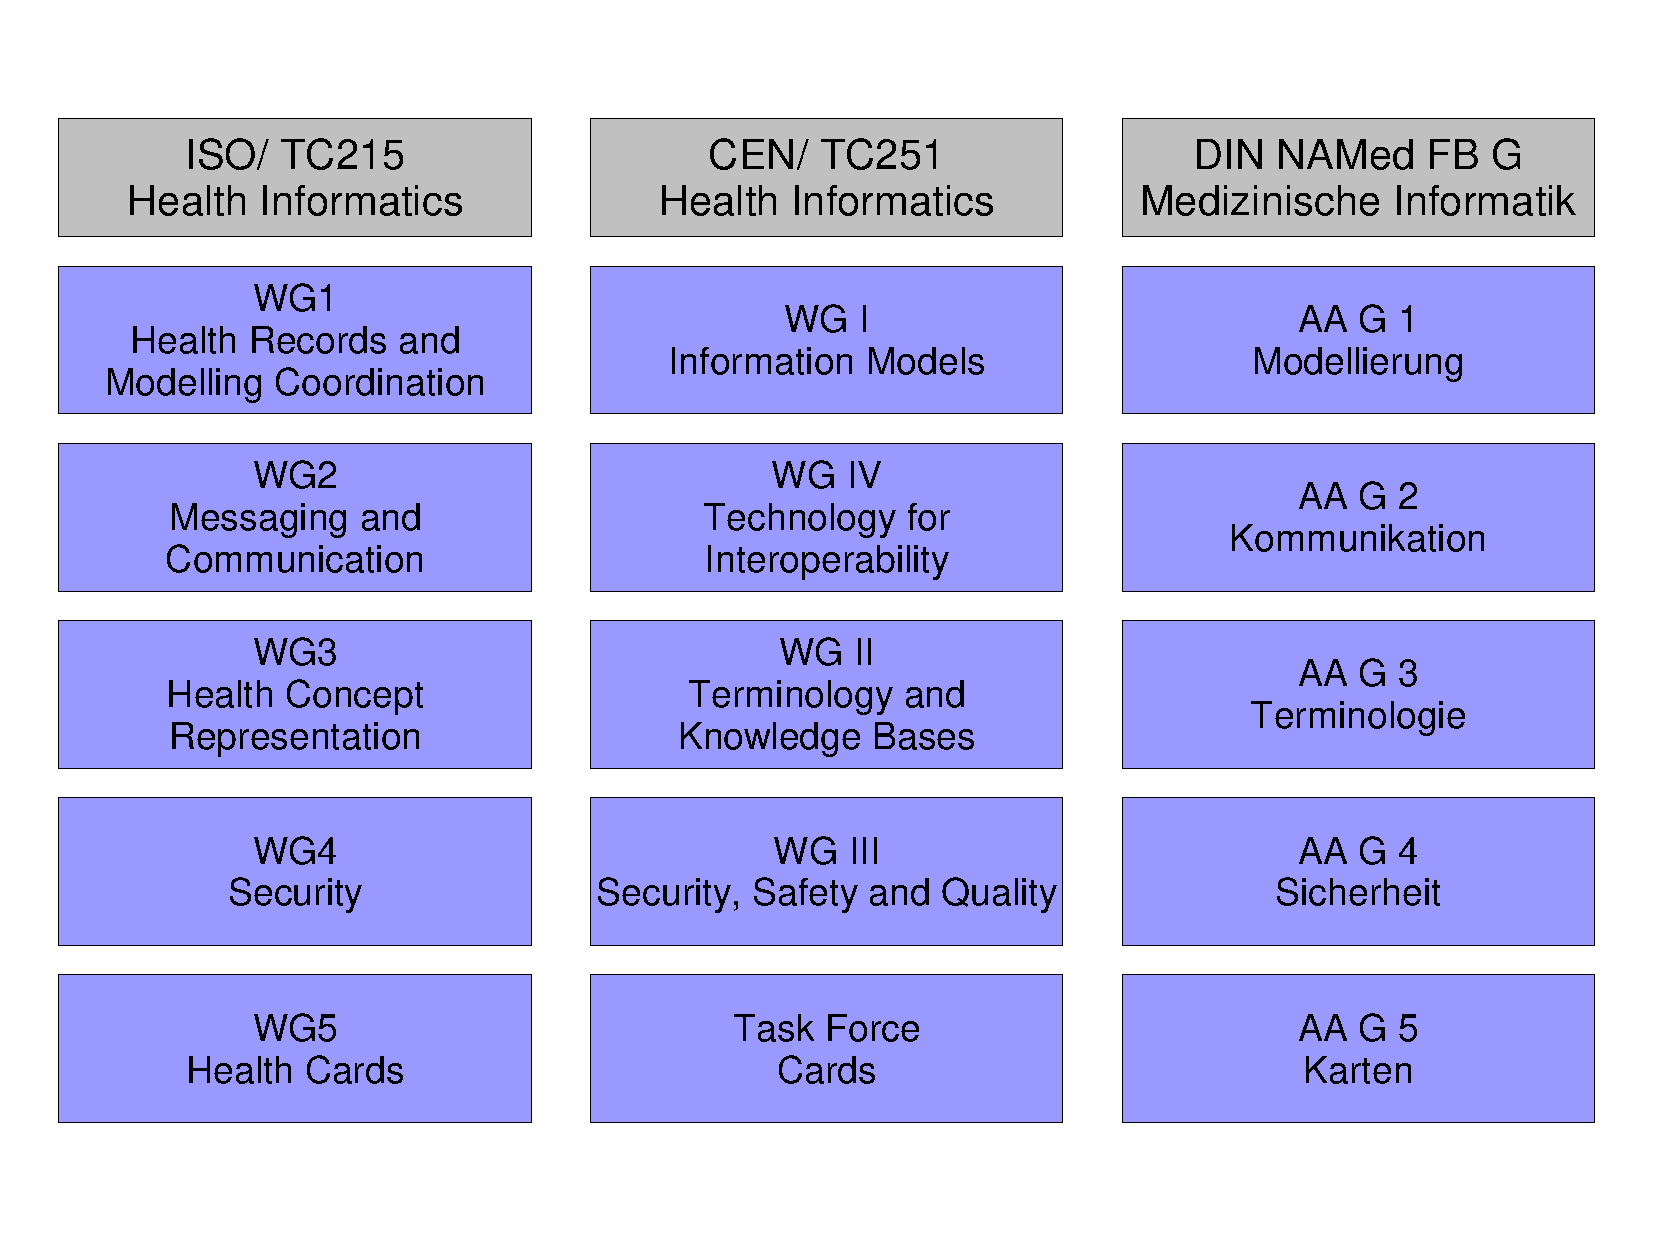
\includegraphics[scale=0.3,angle=-90]{graphic/groups.pdf}
        \caption{Medical Informatics Working Groups of DIN/ CEN/ ISO \cite{atgexpertsreport}}
        \label{groups_figure}
    \end{center}
\end{figure}

The structure of the following sections is chosen after this systematics.
Standards for \emph{Health Record Modelling} will be described first, followed
by those for \emph{Messaging and Communication} and a section on
\emph{Terminology- and Coding Systems}. \emph{Imaging-}, \emph{Health Card-}
and further standards are mentioned afterwards. General remarks on current
\emph{Standards Development Processes} follow. Reflections on the
\emph{Implications} of standards on the development of \emph{Res Medicinae}
will conclude the topic.

%
% $RCSfile: record_modelling.tex,v $
%
% Copyright (C) 2002-2008. Christian Heller.
%
% Permission is granted to copy, distribute and/or modify this document
% under the terms of the GNU Free Documentation License, Version 1.1 or
% any later version published by the Free Software Foundation; with no
% Invariant Sections, with no Front-Cover Texts and with no Back-Cover
% Texts. A copy of the license is included in the section entitled
% "GNU Free Documentation License".
%
% http://www.cybop.net
% - Cybernetics Oriented Programming -
%
% http://www.resmedicinae.org
% - Information in Medicine -
%
% Version: $Revision: 1.1 $ $Date: 2008-08-19 20:41:08 $ $Author: christian $
% Authors: Christian Heller <christian.heller@tuxtax.de>
%

\subsection{Record Modelling}
\label{record_modelling_heading}
\index{Medical Record Modelling Standards}

%
% $RCSfile: cen_tc251.tex,v $
%
% Copyright (C) 2002-2008. Christian Heller.
%
% Permission is granted to copy, distribute and/or modify this document
% under the terms of the GNU Free Documentation License, Version 1.1 or
% any later version published by the Free Software Foundation; with no
% Invariant Sections, with no Front-Cover Texts and with no Back-Cover
% Texts. A copy of the license is included in the section entitled
% "GNU Free Documentation License".
%
% http://www.cybop.net
% - Cybernetics Oriented Programming -
%
% http://www.resmedicinae.org
% - Information in Medicine -
%
% Version: $Revision: 1.1 $ $Date: 2008-08-19 20:41:05 $ $Author: christian $
% Authors: Christian Heller <christian.heller@tuxtax.de>
%

\subsubsection{CEN/TC251}
\label{cen_tc251_heading}
\index{CEN/TC251}
\index{European Committee for Standardization}
\index{CEN}
\index{Standards Development Organisation}
\index{SDO}
\index{Electronic Health Record}
\index{EHR}
\index{Technical Committee 251}
\index{TC251}
\index{ENV 12265}
\index{ENV 13606}
\index{General Purpose Information Component}
\index{GPIC}
\index{EHR Communications Task Force}
\index{EHRcom Task Force}
\index{OpenEHR Archetype}
\index{HL7 CDA}

The \emph{European Committee for Standardization} (CEN) as association of
national \emph{Standards Development Organisations} (SDO) is working on
technical specifications for an \emph{Electronic Health Record} (EHR). The
\emph{Technical Committee} (TC) dealing with that task and medical informatics
in general carries the name \emph{TC251} \cite{centc251}.

While its pre-standard \emph{ENV 12265}, defined in 1995, focused on the EHR
\emph{Architecture}, the successor pre-standard \emph{ENV 13606}, published in
1999, placed more emphasis on \emph{Communication}. Among other things, it
defined a set of reusable components (compositions) called
\emph{General Purpose Information Component} (GPIC) \cite{marley}.
The \emph{ENV 13606} pre-standard consisted of four parts:

\begin{enumerate}
    \item Extended Architecture
    \item Domain Termlist
    \item Distribution Rules
    \item Messages for the Exchange of Information
\end{enumerate}

A third effort, the \emph{EHR Communications} (EHRcom) task force, set up in
December 2001, is to refine \emph{ENV 13606} and to propose a revision that
could be adopted by CEN as formal standard (EN), during 2004. Its current
activities, as described in \cite{ehrcom}, happen in five areas:

\begin{enumerate}
    \item \emph{Reference Model:} generic information model for EHR
        communication
    \item \emph{Archetype Interchange Specification:} generic language for EHR
        representation and communication
    \item \emph{Reference Archetypes and Term Lists:} range of templates
        reflecting clinical requirements and settings
    \item \emph{Security Features:} concepts to enable interaction with
        security components
    \item \emph{Exchange Models:} set of models that can form the basis of
        message-based or service-based communication
\end{enumerate}

\emph{EHRcom} places special focus on the \emph{Harmonisation} of different
standardisation efforts \cite{kalra2002} like CEN's \emph{GPIC}s, openEHR's
\emph{Archetypes} or HL7's \emph{CDA}, described in a later section. But this
is not an easy task. Bert Verhees, for example, reports \cite{openehrtechnical}
about name clashes between the reserved words of many programming languages and
HL7 data types (Set, Array) which made it impossible to use the standard as is
and necessitated a renaming of those types (into something like \emph{HL7Set}
and \emph{HL7Array}). In his opinion, a standard should be platform independent
(operating system- and programming language wise). Thomas Beale of openEHR
writes to this topic \cite{openehrtechnical}:

\begin{quote}
    \ldots\ almost all the issues \ldots\ are actually due to the HL7 data
    types, which CEN unfortunately decided to adopt/ adapt a long time ago. Tom
    Marley and others have struggled to find a version of them which a) remains
    faithful to the idea of HL7 but b) fixes some problems, like strange
    inheritance. Personally, \ldots\ I don't find the HL7 data types a good
    design at all \ldots\ and have made available the reasons in various
    standards discussions, along with many others who have pointed out the same
    problems. The result of this recently has been \ldots\ a new ISO work item
    called \emph{Data Types for Clinical Informatics} \ldots\ which will
    recognise three layers:

    \begin{enumerate}
        \item Inbuilt types (like in ISO 11404)
        \item General purpose clinical types (specified from requirements)
        \item Bindings to particular model systems (such as HL7)
    \end{enumerate}
\end{quote}

%
% $RCSfile: open_ehr.tex,v $
%
% Copyright (C) 2002-2008. Christian Heller.
%
% Permission is granted to copy, distribute and/or modify this document
% under the terms of the GNU Free Documentation License, Version 1.1 or
% any later version published by the Free Software Foundation; with no
% Invariant Sections, with no Front-Cover Texts and with no Back-Cover
% Texts. A copy of the license is included in the section entitled
% "GNU Free Documentation License".
%
% http://www.cybop.net
% - Cybernetics Oriented Programming -
%
% http://www.resmedicinae.org
% - Information in Medicine -
%
% Version: $Revision: 1.1 $ $Date: 2008-08-19 20:41:08 $ $Author: christian $
% Authors: Christian Heller <christian.heller@tuxtax.de>
%

\subsubsection{Open EHR}
\label{open_ehr_heading}
\index{Open Electronic Health Record}
\index{openEHR}
\index{Good European/ Electronic Health Record}
\index{GEHR}
\index{Dual Model Approach}
\index{Archetype}

The \emph{Open Electronic Health Record} (openEHR) \cite{openehr} initiative,
previously called the \emph{Good European/ Electronic Health Record} (GEHR),
arose from a European standardisation effort but is now based in Australia.

Pursueing an idea named the \emph{Dual Model Approach} (section
\ref{dual_model_approach_heading}), which uses a \emph{Meta-Level Architecture}
as described by the \emph{Reflection} pattern (section \ref{reflection_heading}),
it wants to specify so-called \emph{Archetypes} -- formally specified knowledge
templates of requirements for representing and communicating EHR information.

The effort is based on the idea of no-cost open standards and free contribution.


%
% $RCSfile: messaging_and_communication.tex,v $
%
% Copyright (C) 2002-2008. Christian Heller.
%
% Permission is granted to copy, distribute and/or modify this document
% under the terms of the GNU Free Documentation License, Version 1.1 or
% any later version published by the Free Software Foundation; with no
% Invariant Sections, with no Front-Cover Texts and with no Back-Cover
% Texts. A copy of the license is included in the section entitled
% "GNU Free Documentation License".
%
% http://www.cybop.net
% - Cybernetics Oriented Programming -
%
% http://www.resmedicinae.org
% - Information in Medicine -
%
% Version: $Revision: 1.1 $ $Date: 2008-08-19 20:41:07 $ $Author: christian $
% Authors: Christian Heller <christian.heller@tuxtax.de>
%
\subsection{Messaging and Communication}
\label{messaging_and_communication_heading}
\index{Medical Messaging and Communication Standards}
%
% $RCSfile: health_level_seven.tex,v $
%
% Copyright (C) 2002-2008. Christian Heller.
%
% Permission is granted to copy, distribute and/or modify this document
% under the terms of the GNU Free Documentation License, Version 1.1 or
% any later version published by the Free Software Foundation; with no
% Invariant Sections, with no Front-Cover Texts and with no Back-Cover
% Texts. A copy of the license is included in the section entitled
% "GNU Free Documentation License".
%
% http://www.cybop.net
% - Cybernetics Oriented Programming -
%
% http://www.resmedicinae.org
% - Information in Medicine -
%
% Version: $Revision: 1.1 $ $Date: 2008-08-19 20:41:07 $ $Author: christian $
% Authors: Christian Heller <christian.heller@tuxtax.de>
%

\subsubsection{Health Level Seven}
\label{health_level_seven_heading}
\index{Health Level Seven}
\index{HL7}
\index{Reference Information Model}
\index{RIM}
\index{Clinical Document Architecture}
\index{CDA}
\index{XML}
\index{Common Message Element Type}
\index{CMET}
\index{Refined Message Information Model}
\index{RMIM}
\index{Hospital Information System}
\index{HIS}
\index{Practice Management System}
\index{PMS}

\emph{Health Level Seven} (HL7), as it describes itself \cite{hl7}, is:
\textit{a not-for-profit, ANSI-accredited standards developing organization
dedicated to providing a comprehensive framework and related standards for the
exchange, integration, sharing, and retrieval of electronic health information
that supports clinical practice and the management, delivery and evaluation of
health services.} The more than 2000 individuals representing over 500
corporate members, world-wide, do for a great part belong to healthcare
industry, implementing its interests. Accordingly, HL7's endeavors are
sponsored, in part, by that industry. Its name \emph{Level Seven}, after
\cite{rogers}, refers to the highest level of the ISO OSI communication model
(section \ref{systems_interconnection_heading}).

Besides the mentioned framework called \emph{Reference Information Model} (RIM),
the organisation worked out a number of specifications for the exchange of messages
and documents, newer formats being the \emph{Clinical Document Architecture} (CDA),
an XML-only specification, and the \emph{Common Message Element Type} (CMET)
\cite{marley}, a reusable component.

Thomas Beale criticised in \cite{openhealth}, that CDA did not have very strong
semantics for some of its detailed parts, since they were derived from XHTML,
and that it tended to mix presentation and representation concerns somewhat.
Furthermore, CDA had recently incorporated some RIM classes into its content
level, via the creation of a \emph{Refined Message Information Model} (RMIM)
which were a pity, because it reduced its genericness and made it dependend on
the RIM, which were essentially an analysis pattern of domain relationships,
not a model of recording.

Instead, as Beale writes in a later message to \cite{openhealth}, they (HL7)
might start thinking about generic solutions, which incorporate clinical
models, separated from their XML schemas, for a start. \ldots\ Single level XML
approaches didn't have much long term future in his opinion, because they
didn't properly separate clinical models from information representation, which
were required to allow compositional clinical models and specialisable clinical
models to be built independently from the software.

HL7's recommendations found partly application in a greater number of
\emph{Hospital Information Systems} (HIS), but rarely in smaller or
medium-sized \emph{Practice Management Systems} (PMS).

%
% $RCSfile: healthcare_domain_task_force.tex,v $
%
% Copyright (C) 2002-2008. Christian Heller.
%
% Permission is granted to copy, distribute and/or modify this document
% under the terms of the GNU Free Documentation License, Version 1.1 or
% any later version published by the Free Software Foundation; with no
% Invariant Sections, with no Front-Cover Texts and with no Back-Cover
% Texts. A copy of the license is included in the section entitled
% "GNU Free Documentation License".
%
% http://www.cybop.net
% - Cybernetics Oriented Programming -
%
% http://www.resmedicinae.org
% - Information in Medicine -
%
% Version: $Revision: 1.1 $ $Date: 2008-08-19 20:41:07 $ $Author: christian $
% Authors: Christian Heller <christian.heller@tuxtax.de>
%

\subsubsection{Healthcare Domain Task Force}
\label{healthcare_domain_task_force_heading}
\index{Object Management Group}
\index{OMG}
\index{Model Driven Architecture}
\index{MDA}
\index{Common Object Request Broker Architecture}
\index{CORBA}
\index{Interface Definition Language}
\index{IDL}
\index{Object Request Broker}
\index{ORB}
\index{Internet Inter ORB Protocol}
\index{IIOP}
\index{Healthcare Domain Taskforce}
\index{HDTF}
\index{CORBAmed}
\index{Person (Patient) Identification Service}
\index{PIDS}
\index{Lexicon (Terminology) Query Service}
\index{LQS}
\index{Clinical Observations Access Service}
\index{COAS}
\index{Resource Access Decision Service}
\index{RADS}
\index{Clinical Image Access Service}
\index{CIAS}

The \emph{Object Management Group} (OMG) whose mission is: \textit{to help
computer users solve integration problems by supplying open, vendor-neutral
interoperability specifications}, is the creator of widely-used de facto
standards (section \ref{model_driven_architecture_heading}) like UML, MOF, XMI,
CWM or CORBA, all now belonging to the \emph{Model Driven Architecture} (MDA).

Published in the 1990s, the \emph{Common Object Request Broker Architecture}
(CORBA) was one of the first standards specifications created by the OMG. It
tried to separate interfaces of programming objects (components) from their
implementation, to improve communication between programs, independent of which
programming language, operating system, computer architecture or network were
used. The specification includes the neutral \emph{Interface Definition Language}
(IDL), the \emph{Object Request Broker} (ORB) middleware functionality and a
corresponding \emph{Internet Inter ORB Protocol} (IIOP).

CORBA has been adopted by many applications, and been adapted for many domains,
one of them being \emph{Healthcare}. The OMG working group dealing with that
field is the \emph{Healthcare Domain Taskforce} (HDTF) \cite{omghdtf} (formerly
called \emph{CORBAmed}). It defined IDL interfaces for a number of different
healthcare services, for example:

\begin{itemize}
    \item[-] \emph{Person (Patient) Identification Service} (PIDS)
    \item[-] \emph{Lexicon (Terminology) Query Service} (LQS)
    \item[-] \emph{Clinical Observations Access Service} (COAS)
    \item[-] \emph{Resource Access Decision Service} (RADS)
    \item[-] \emph{Clinical Image Access Service} (CIAS)
\end{itemize}

HDTF specifications are helpful in that they standardise certain functionality
calls that all systems implementing the corresponding interfaces may rely on.
However, they do not make any assertions about how medical knowledge should be
structured.

%
% $RCSfile: edifact.tex,v $
%
% Copyright (C) 2002-2008. Christian Heller.
%
% Permission is granted to copy, distribute and/or modify this document
% under the terms of the GNU Free Documentation License, Version 1.1 or
% any later version published by the Free Software Foundation; with no
% Invariant Sections, with no Front-Cover Texts and with no Back-Cover
% Texts. A copy of the license is included in the section entitled
% "GNU Free Documentation License".
%
% http://www.cybop.net
% - Cybernetics Oriented Programming -
%
% http://www.resmedicinae.org
% - Information in Medicine -
%
% Version: $Revision: 1.1 $ $Date: 2008-08-19 20:41:06 $ $Author: christian $
% Authors: Christian Heller <christian.heller@tuxtax.de>
%

\subsubsection{EDIFACT}
\label{edifact_heading}
\index{Electronic Data Interchange for Administration, Commerce and Transport}
\index{EDIFACT}
\index{United Nations Standard}
\index{UN Standard}
\index{European Board of EDI Standardisation}
\index{EBES}
\index{EBES Expert Group 9}
\index{EEG9}
\index{ISO 9735}

The \emph{Electronic Data Interchange for Administration, Commerce and Transport}
(EDIFACT) \cite{edifact} is a standard maintained by committees of the
\emph{United Nations} (UN). It was defined to ease the electronic exchange of
general business data, but is widely used for the transmission of healthcare
information between organisations, too. \cite{kalra1998}

The \emph{European Board of EDI Standardisation} (EBES) participates in the
development and distribution of EDIFACT standards. For the healthcare sector,
this task falls to the \emph{EBES Expert Group} (EEG) 9. It has specified many
message formats, for instance for referral letters or electronic prescriptions.
Although some countries like Denmark, Norway or Austria make use of these
standards, they have not gained wider currency. \cite{atgexpertsreport}

Messages in form of the EDIFACT protocol are based on syntax elements which are
described in another standard, the \emph{ISO 9735}. Their data elements are
contained in a well-defined collection of segments, in a well-defined sequence.
\cite{edifactory}

%
% $RCSfile: x_data_carrier.tex,v $
%
% Copyright (C) 2002-2008. Christian Heller.
%
% Permission is granted to copy, distribute and/or modify this document
% under the terms of the GNU Free Documentation License, Version 1.1 or
% any later version published by the Free Software Foundation; with no
% Invariant Sections, with no Front-Cover Texts and with no Back-Cover
% Texts. A copy of the license is included in the section entitled
% "GNU Free Documentation License".
%
% http://www.cybop.net
% - Cybernetics Oriented Programming -
%
% http://www.resmedicinae.org
% - Information in Medicine -
%
% Version: $Revision: 1.1 $ $Date: 2008-08-19 20:41:09 $ $Author: christian $
% Authors: Christian Heller <christian.heller@tuxtax.de>
%

\subsubsection{x Data Carrier}
\label{x_data_carrier_heading}
\index{x Data Carrier}
\index{x Datentr\"{a}ger}
\index{xDT}
\index{EDI}
\index{Datentr\"{a}ger}
\index{DT}
\index{German College of Community Physicians}
\index{Kassen\"{a}rztliche Bundesvereinigung}
\index{KBV}
\index{Behandlungs Datentr\"{a}ger}
\index{BDT}
\index{Labor Datentr\"{a}ger}
\index{LDT}
\index{Abrechnungs Datentr\"{a}ger}
\index{ADT}
\index{Ambulant Operieren Datentr\"{a}ger}
\index{AODT}
\index{Geraete Datentr\"{a}ger}
\index{GDT}
\index{Kommunikations Datentr\"{a}ger}
\index{KDT}
\index{Kassenaerztliche Vereinigung Datentr\"{a}ger}
\index{KVDT}
\index{Practice Management System}
\index{PMS}
\index{General Practitioners}
\index{GP}
\index{Hospital Information System}
\index{HIS}
\index{HL7}
\index{KV Nordrhein}
\index{Zentralinstitut f\"{u}r die Kassen\"{a}rztliche Versorgung}
\index{ZI}
\index{Deutsches Institut f\"{u}r Medizinische Dokumentation und Information}
\index{DIMDI}
\index{Bundesvereinigung Deutscher Apotheker Verb\"{a}nde}
\index{ABDA}
\index{Verband der Hersteller von IT L\"{o}sungen f\"{u}r das Gesundheitswesen}
\index{VHitG}
\index{Verband Deutscher Arztpraxis Softwarehersteller}
\index{VDAP}
\index{Qualit\"{a}tsring Medizinische Software}
\index{QMS}
\index{Standardisation of Communication between Information Systems in Physician's Offices and Hospitals using XML}
\index{SCIPHOX}
\index{XML}
\index{CDA}
\index{Robert Koch Institut}
\index{RKI}
\index{Studienzentrum G\"{o}ttingen (Allgemeinmedizin)}

Various national standards for medical software exist. In Germany, a widely
used de facto standard for EDI in healthcare is the \emph{x Datentr\"{a}ger}
(xDT) \cite{xdt}, a family of formats specifying data packets. The German word
\emph{Datentr\"{a}ger} (DT) means something like \emph{Data Container}. The
\emph{German College of Community Physicians}, called \emph{Kassen\"{a}rztliche
Bundesvereinigung} (KBV), is initiator and maintainer of xDT, to which belong,
for example:

\begin{itemize}
    \item[-] \emph{Behandlungs DT} (BDT): EHR interchange between systems
        (was ADT and developed to the current BDT)
    \item[-] \emph{Labor DT} (LDT): laboratory data format
        (predecessor: \emph{Bonner Modell})
    \item[-] \emph{Abrechnungs DT} (ADT): reimbursement data format
    \item[-] \emph{Ambulant Operieren DT} (AODT): outpatient/ minor surgery
        data format
    \item[-] \emph{Ger\"{a}te DT} (GDT): medical device interfacing
        (predecessor: \emph{M\"{u}nchener Protokoll})
    \item[-] \emph{Kommunikations DT} (KDT): communications data format
        (referrral letters)
    \item[-] \emph{Kassen\"{a}rztliche Vereinigung DT} (KVDT): all sorts of
        reimbursement data (container format to wrap the others)
\end{itemize}

After Karsten Hilbert \cite{openhealth}, xDT were mostly used in
\emph{Practice Management Systems} (PMS) of \emph{General Practitioners} (GP).
Most \emph{Hospital Information Systems} (HIS) weren't using it. Some lab
software being part of a HIS and servicing PMS apparently would use it.

Besides the KBV, institutions and groups like HL7, \emph{KV Nordrhein},
\emph{Zentralinstitut f\"{u}r die Kassen\"{a}rztliche Versorgung} (ZI),
\emph{Deutsches Institut f\"{u}r Medizinische Dokumentation und Information}
(DIMDI), \emph{Bundesvereinigung Deutscher Apotheker Verb\"{a}nde} (ABDA),
\emph{Verband der Hersteller von IT L\"{o}sungen f\"{u}r das Gesundheitswesen}
(VHitG), \emph{Verband Deutscher Arztpraxis Softwarehersteller} (VDAP) and
\emph{Qualit\"{a}tsring Medizinische Software} (QMS) are currently working on
converting xDT into an XML-based standard, called \emph{Standardisation of
Communication between Information Systems in Physician's Offices and Hospitals
using XML} (SCIPHOX) \cite{sciphox}, which originates in HL7's CDA. Accompanying
projects \cite{medvip} include the \emph{Robert Koch Institut} (RKI),
\emph{Studienzentrum G\"{o}ttingen} (Allgemeinmedizin) and others, as further
partners.

%
% $RCSfile: healthcare_xchange_protocol.tex,v $
%
% Copyright (C) 2002-2008. Christian Heller.
%
% Permission is granted to copy, distribute and/or modify this document
% under the terms of the GNU Free Documentation License, Version 1.1 or
% any later version published by the Free Software Foundation; with no
% Invariant Sections, with no Front-Cover Texts and with no Back-Cover
% Texts. A copy of the license is included in the section entitled
% "GNU Free Documentation License".
%
% http://www.cybop.net
% - Cybernetics Oriented Programming -
%
% http://www.resmedicinae.org
% - Information in Medicine -
%
% Version: $Revision: 1.1 $ $Date: 2008-08-19 20:41:07 $ $Author: christian $
% Authors: Christian Heller <christian.heller@tuxtax.de>
%

\subsubsection{Healthcare Xchange Protocol}
\label{healthcare_xchange_protocol_heading}
\index{Healthcare Xchange Protocol}
\index{HXP}
\index{Open Source Software}
\index{OSS}
\index{XML}
\index{Remote Procedure Call}
\index{RPC}

Finally, there are standardisation activities in the \emph{Open Source Software}
(OSS) community. Just recently, the \emph{Healthcare Xchange Protocol} (HXP)
\cite{hxp} was defined by a number of projects.

HXP is a data exchange protocol to be used by healthcare applications to
communicate transparently with each other, regardless of their corresponding
platform. The aim is to make data exchange simple to implement, easy to
understand, flexible, reliable, secure, free, and more. HXP is based upon the
XML \emph{Remote Procedure Call} (RPC) open standards specifications, that is
it uses messages in XML format for communication.

The specification and all documentation are open and everybody can contribute
ideas.


%
% $RCSfile: terminology_systems.tex,v $
%
% Copyright (C) 2002-2008. Christian Heller.
%
% Permission is granted to copy, distribute and/or modify this document
% under the terms of the GNU Free Documentation License, Version 1.1 or
% any later version published by the Free Software Foundation; with no
% Invariant Sections, with no Front-Cover Texts and with no Back-Cover
% Texts. A copy of the license is included in the section entitled
% "GNU Free Documentation License".
%
% http://www.cybop.net
% - Cybernetics Oriented Programming -
%
% http://www.resmedicinae.org
% - Information in Medicine -
%
% Version: $Revision: 1.1 $ $Date: 2008-08-19 20:41:09 $ $Author: christian $
% Authors: Christian Heller <christian.heller@tuxtax.de>
%

\subsection{Terminology Systems}
\label{terminology_systems_heading}
\index{Medical Terminology Systems}
\index{Enumerative Scheme}
\index{Compositional Scheme}
\index{Lexical Scheme}

Besides defining the differences between a \emph{Lexicon} (list of pure words)
and \emph{Terminology} (also containing phrases), the latter sometimes called
\emph{Vocabulary}, section \ref{terminology_heading} introduced tree-like
\emph{Hierarchies} as one way to organise such sets of words or terms. Three
concrete schemes for organising terminologies were described in section
\ref{schemes_heading}: \emph{Enumerative}, \emph{Compositional} and
\emph{Lexical}. Controversial opinions about terminologies exist. Thomas Beale
wrote in \cite[December 2003]{openhealth}:

\begin{quote}
    \ldots\ trying to standardise the whole of medicine \ldots\ is a fruitless
    enterprise. Sam Heard has said this many times in presentations in
    Australia, and when he first started saying it, was amazed not to be
    stoned publicly; in fact many people have come to this conclusion through
    their own hard work, but aren't comfortable with saying it, since it goes
    against current orthodoxy (embodied in things like SNOMED CT).
\end{quote}

Nevertheless, terminologies \emph{are} a topic of research and sometimes used
in practice, as the example of ICD (see below) shows. This section therefore
briefly describes some medical terminologies and, by referring to Jeremy Rogers
\cite{rogers}, tries to assign them to one of the before-mentioned schemes.

%
% $RCSfile: icd.tex,v $
%
% Copyright (C) 2002-2008. Christian Heller.
%
% Permission is granted to copy, distribute and/or modify this document
% under the terms of the GNU Free Documentation License, Version 1.1 or
% any later version published by the Free Software Foundation; with no
% Invariant Sections, with no Front-Cover Texts and with no Back-Cover
% Texts. A copy of the license is included in the section entitled
% "GNU Free Documentation License".
%
% http://www.cybop.net
% - Cybernetics Oriented Programming -
%
% http://www.resmedicinae.org
% - Information in Medicine -
%
% Version: $Revision: 1.1 $ $Date: 2008-08-19 20:41:07 $ $Author: christian $
% Authors: Christian Heller <christian.heller@tuxtax.de>
%

\subsubsection{ICD}
\label{icd_heading}
\index{International Classification of Diseases}
\index{ICD}
\index{World Health Organisation}
\index{WHO}

The \emph{International Classification of Diseases} (ICD): \textit{has become
the international standard diagnostic classification for all general
epidemiological and many health management purposes \ldots\ It is used to
classify diseases and other health problems recorded on many types of health
and vital records including death certificates and hospital records.} \cite{icd}

Scheme: enumerative\\
Maintainer: World Health Organisation (WHO)

%
% $RCSfile: opcs.tex,v $
%
% Copyright (C) 2002-2008. Christian Heller.
%
% Permission is granted to copy, distribute and/or modify this document
% under the terms of the GNU Free Documentation License, Version 1.1 or
% any later version published by the Free Software Foundation; with no
% Invariant Sections, with no Front-Cover Texts and with no Back-Cover
% Texts. A copy of the license is included in the section entitled
% "GNU Free Documentation License".
%
% http://www.cybop.net
% - Cybernetics Oriented Programming -
%
% http://www.resmedicinae.org
% - Information in Medicine -
%
% Version: $Revision: 1.1 $ $Date: 2008-08-19 20:41:08 $ $Author: christian $
% Authors: Christian Heller <christian.heller@tuxtax.de>
%

\subsubsection{OPCS}
\label{opcs_heading}
\index{Office of Population Censuses and Surveys Classification of Surgical Operations and Procedures}
\index{OPCS}
\index{National Health Service Information Authority}
\index{NHSIA}

The \emph{Office of Population Censuses and Surveys Classification of Surgical
Operations and Procedures} (OPCS) is a: \textit{statistical classification of
diseases and surgical procedures, respectively.} It allows the: \textit{logical
translation of clinical statements into codes in a way that facilitates the
retrieval of data in a consistent manner and comparative analysis of aggregated
datasets compiled from multiple sources.} \cite{opcs}

Scheme: enumerative\\
Maintainer: \emph{National Health Service Information Authority} (NHSIA)

%
% $RCSfile: read.tex,v $
%
% Copyright (C) 2002-2008. Christian Heller.
%
% Permission is granted to copy, distribute and/or modify this document
% under the terms of the GNU Free Documentation License, Version 1.1 or
% any later version published by the Free Software Foundation; with no
% Invariant Sections, with no Front-Cover Texts and with no Back-Cover
% Texts. A copy of the license is included in the section entitled
% "GNU Free Documentation License".
%
% http://www.cybop.net
% - Cybernetics Oriented Programming -
%
% http://www.resmedicinae.org
% - Information in Medicine -
%
% Version: $Revision: 1.1 $ $Date: 2008-08-19 20:41:08 $ $Author: christian $
% Authors: Christian Heller <christian.heller@tuxtax.de>
%

\subsubsection{READ}
\label{read_heading}
\index{Read Codes}
\index{READ}
\index{Clinical Terms Version 3}
\index{CTV3}
\index{ICD-10}
\index{OPCS-4}
\index{National Health Service Information Authority}
\index{NHSIA}

The \emph{Read Codes} (READ), as their older name \emph{Clinical Terms Version 3}
(CTV3) says, are a: \textit{list of terms describing the care and treatment of
patients}. They: \textit{cover a wide range of topics in categories such as
signs and symptoms, treatments and therapies, investigations, occupations,
diagnoses and drugs and appliances.} Further, they: \textit{provide cross maps
to both ICD-10 and OPCS-4 classification codes.} \cite{read}

Scheme: enumerative\\
Maintainer: \emph{United Kingdom} (UK)
\emph{National Health Service Information Authority} (NHSIA)

%
% $RCSfile: loinc.tex,v $
%
% Copyright (C) 2002-2008. Christian Heller.
%
% Permission is granted to copy, distribute and/or modify this document
% under the terms of the GNU Free Documentation License, Version 1.1 or
% any later version published by the Free Software Foundation; with no
% Invariant Sections, with no Front-Cover Texts and with no Back-Cover
% Texts. A copy of the license is included in the section entitled
% "GNU Free Documentation License".
%
% http://www.cybop.net
% - Cybernetics Oriented Programming -
%
% http://www.resmedicinae.org
% - Information in Medicine -
%
% Version: $Revision: 1.1 $ $Date: 2008-08-19 20:41:07 $ $Author: christian $
% Authors: Christian Heller <christian.heller@tuxtax.de>
%

\subsubsection{LOINC}
\label{loinc_heading}
\index{Logical Observation Identifiers, Names and Codes}
\index{LOINC}
\index{SNOMED CT}
\index{Regenstrief Institute}

The \emph{Logical Observation Identifiers, Names and Codes} (LOINC) is a
database whose purpose is: \textit{to facilitate the exchange and pooling of
results \ldots\ for clinical care, outcomes management, and research.} Its
codes are: \textit{universal identifiers for laboratory- and other clinical
observations.} \cite{loinc} After \cite{rogers}, it were now closely allied to
SNOMED CT (see later section).

Scheme: hybrid enumerative-compositional\\
Maintainer: \emph{United States} (US) \emph{Regenstrief Institute}

%
% $RCSfile: icnp.tex,v $
%
% Copyright (C) 2002-2008. Christian Heller.
%
% Permission is granted to copy, distribute and/or modify this document
% under the terms of the GNU Free Documentation License, Version 1.1 or
% any later version published by the Free Software Foundation; with no
% Invariant Sections, with no Front-Cover Texts and with no Back-Cover
% Texts. A copy of the license is included in the section entitled
% "GNU Free Documentation License".
%
% http://www.cybop.net
% - Cybernetics Oriented Programming -
%
% http://www.resmedicinae.org
% - Information in Medicine -
%
% Version: $Revision: 1.1 $ $Date: 2008-08-19 20:41:07 $ $Author: christian $
% Authors: Christian Heller <christian.heller@tuxtax.de>
%

\subsubsection{ICNP}
\label{icnp_heading}
\index{International Classification for Nursing Practice}
\index{ICNP}
\index{International Council of Nurses}
\index{ICN}

The \emph{International Classification for Nursing Practice} (ICNP) is a:
\textit{combinatorial terminology for nursing practice that facilitates
crossmapping of local terms and existing vocabularies and classifications.} It
wants to: \textit{establish a common language for describing nursing practice
in order to improve communication among nurses, and between nurses and others.}
\cite{icnp}

Scheme: hybrid enumerative-compositional\\
Maintainer: \emph{International Council of Nurses} (ICN)

%
% $RCSfile: snomed_ct.tex,v $
%
% Copyright (C) 2002-2008. Christian Heller.
%
% Permission is granted to copy, distribute and/or modify this document
% under the terms of the GNU Free Documentation License, Version 1.1 or
% any later version published by the Free Software Foundation; with no
% Invariant Sections, with no Front-Cover Texts and with no Back-Cover
% Texts. A copy of the license is included in the section entitled
% "GNU Free Documentation License".
%
% http://www.cybop.net
% - Cybernetics Oriented Programming -
%
% http://www.resmedicinae.org
% - Information in Medicine -
%
% Version: $Revision: 1.1 $ $Date: 2008-08-19 20:41:08 $ $Author: christian $
% Authors: Christian Heller <christian.heller@tuxtax.de>
%

\subsubsection{SNOMED CT}
\label{snomed_ct_heading}
\index{Systematized Nomenclature of Medicine}
\index{SNOMED}
\index{SNOMED Clinical Terms}
\index{SNOMED CT}
\index{SNOMED Reference Terminology}
\index{SNOMED RT}
\index{Read Codes}
\index{READ}
\index{ICD-9-CM}
\index{ICD-10}
\index{ICD-03}
\index{OPCS-4}
\index{LOINC}
\index{SNOMED International}
\index{College of American Pathologists}
\index{CAP}

The \emph{Systematized Nomenclature of Medicine} (SNOMED) \emph{Clinical Terms}
(SNOMED CT) is: \textit{a dynamic, scientifically validated clinical health care
terminology and infrastructure that makes health care knowledge more usable and
accessible.} The SNOMED CT core terminology: \textit{contains over 364,400
health care concepts with unique meanings and formal logic-based definitions
organized into hierarchies. As of January 2005, the fully populated table with
unique descriptions for each concept contains more than 984,000 descriptions.
Approximately 1.45 million semantic relationships exist to enable reliability
and consistency of data retrieval.} \cite{snomed}

SNOMED CT was created by combining the content and structure of the SNOMED
\emph{Reference Terminology} (SNOMED RT) with the United Kingdom's (UK)
\emph{Read Codes} (READ) clinical terms. Meanwhile, mappings and integrations
for further standards exist, e.g. for several ICD versions (ICD-9-CM, ICD-10,
ICD-O3), OPCS-4 and LOINC.

Scheme: hybrid enumerative-compositional\\
Maintainer: \emph{SNOMED International} and \emph{College of American Pathologists} (CAP)

==

--- Klaus Veil <klaus@veil.net.au> wrote:

> Nandalal,
> �
> The concerns about closedness and excessive cost were indeed the main
> drivers that finally convinced CAP in the USA that an "open" international
> Standards Development Organisation was the only viable way forward. �CAP
> have committed to transfer the SNOMED IP to the new SDO.
> �
> Klaus
> 
> � _____ �
> 
> From: openhealth@yahoogroups.com [mailto:openhealth@yahoogroups.com] On
> Behalf Of Nandalal Gunaratne
> Sent: Monday, 5 February 2007 20:06
> To: openhealth@yahoogroups.com
> Subject: RE: [openhealth] OSHCA Conference Topics
> 
> 
> 
> Klaus,
> 
> Most of asia use ICD and other WHO standards. SNOMED
> is considered too expensive and too closed. I hope the
> new initiative would change that.
> 
> Nandalal

%
% $RCSfile: odyssee.tex,v $
%
% Copyright (C) 2002-2008. Christian Heller.
%
% Permission is granted to copy, distribute and/or modify this document
% under the terms of the GNU Free Documentation License, Version 1.1 or
% any later version published by the Free Software Foundation; with no
% Invariant Sections, with no Front-Cover Texts and with no Back-Cover
% Texts. A copy of the license is included in the section entitled
% "GNU Free Documentation License".
%
% http://www.cybop.net
% - Cybernetics Oriented Programming -
%
% http://www.resmedicinae.org
% - Information in Medicine -
%
% Version: $Revision: 1.1 $ $Date: 2008-08-19 20:41:07 $ $Author: christian $
% Authors: Christian Heller <christian.heller@tuxtax.de>
%

\subsubsection{Odyssee}
\label{odyssee_heading}
\index{Odyssee}
\index{Logiciel Nautilus}

The \emph{Odyssee} open source project \cite{nautilus} contains a terminology
(\emph{Lexique}) of more than 35,000 (French) terms, each with a code, at the
core of its system. Additionally, it contains a \emph{Semantic Network} of
links between terms of the Lexique, to give sense. Links can be \emph{is a},
\emph{belongs to} or \emph{has unit}. Philippe Ameline writes
\cite{openehrtechnical}:

\begin{quotation}
    In Odyssee, we describe all that we can with trees. If we compare the
    Lexique with medical vocabulary, trees are sentences made of its words.
    Each node of a tree is an object with fields like the Lexique's code,
    complement (to store numbers or external codes), degree of evidence (from
    0=no to 100=certain). Trees can also contain free text sentences \ldots

    In Odyssee, each and every structured document is a tree; you just have to
    look at the Lexique term at its root to know what it is. The whole patient
    record can even be seen as a huge tree with (the) term \emph{Patient} as
    root. Trees can be shown \emph{as is} or, for report generation, be
    translated to natural langage sentences.
\end{quotation}

Scheme: compositional\\
Maintainer: Odyssee \emph{Non-Profit Organisation} (NPO), \emph{Logiciel Nautilus}

%
% $RCSfile: open_galen.tex,v $
%
% Copyright (C) 2002-2008. Christian Heller.
%
% Permission is granted to copy, distribute and/or modify this document
% under the terms of the GNU Free Documentation License, Version 1.1 or
% any later version published by the Free Software Foundation; with no
% Invariant Sections, with no Front-Cover Texts and with no Back-Cover
% Texts. A copy of the license is included in the section entitled
% "GNU Free Documentation License".
%
% http://www.cybop.net
% - Cybernetics Oriented Programming -
%
% http://www.resmedicinae.org
% - Information in Medicine -
%
% Version: $Revision: 1.1 $ $Date: 2008-08-19 20:41:08 $ $Author: christian $
% Authors: Christian Heller <christian.heller@tuxtax.de>
%

\subsubsection{OpenGALEN}
\label{open_galen_heading}
\index{Generalised Architecture for Languages, Encyclopedias and Nomenclatures in Med.}
\index{GALEN}
\index{GALEN Common Reference Model}
\index{GALEN CRM}
\index{GALEN Representation and Integration Language}
\index{GRAIL}
\index{OpenGALEN}
\index{Synergy on the Extranet}
\index{SynEx}
\index{Synapses}

The \emph{Generalised Architecture for Languages, Encyclopaedias and
Nomenclatures in Medicine} (GALEN) is trying to construct a:
\textit{semantically sound model of clinical terminology} -- the GALEN
\emph{Common Reference Model} (CRM). The formal rules (representation scheme)
for manipulating its concepts are provided by the \emph{GALEN Representation
and Integration Language} (GRAIL).

The original GALEN project was sponsored by the \emph{European Union} (EU) and
open-sourced and renamed into \emph{OpenGALEN}, in 1999. It later continued as
part of the \emph{Synergy on the Extranet} (SynEx) project \cite{synex}, which
arose from the \emph{Synapses} project aiming at implementing a federated
healthcare record server.

Scheme: compositional\\
Maintainer: OpenGALEN \emph{Non-Profit Organisation} (NPO)

%
% $RCSfile: umls.tex,v $
%
% Copyright (C) 2002-2008. Christian Heller.
%
% Permission is granted to copy, distribute and/or modify this document
% under the terms of the GNU Free Documentation License, Version 1.1 or
% any later version published by the Free Software Foundation; with no
% Invariant Sections, with no Front-Cover Texts and with no Back-Cover
% Texts. A copy of the license is included in the section entitled
% "GNU Free Documentation License".
%
% http://www.cybop.net
% - Cybernetics Oriented Programming -
%
% http://www.resmedicinae.org
% - Information in Medicine -
%
% Version: $Revision: 1.1 $ $Date: 2008-08-19 20:41:09 $ $Author: christian $
% Authors: Christian Heller <christian.heller@tuxtax.de>
%

\subsubsection{UMLS}
\label{umls_heading}
\index{Unified Medical Language System}
\index{UMLS}
\index{UMLS Metathesaurus}
\index{Medical Subject Headings}
\index{MeSH}
\index{UMLS Semantic Network}
\index{UMLS Specialist Lexicon}
\index{UMLS Knowledge Source Server}
\index{UMLSKS}
\index{National Library of Medicine}
\index{NLM}

The \emph{Unified Medical Language System} (UMLS) consists of knowledge sources
(databases) and associated software tools (programs). By design, the knowledge
sources are multi-purpose, that is: \textit{they are not optimised for particular
applications, but can be applied in systems that perform a range of functions
involving one or more types of information, e.g. patient records, scientific
literature, guidelines, public health data.} \cite{umls} There are three UMLS
knowledge sources:

\begin{itemize}
    \item[-] \emph{Metathesaurus:} a very large, multi-purpose, and
        multi-lingual vocabulary database containing information about
        biomedical and health-related concepts, their various names, and the
        relationships among them; its source vocabularies are many different
        thesauri, classifications, code sets, and lists of controlled terms, of
        which it cross-references over 79 \cite{rogers}, often by deriving from
        lexical analysis of the terms; a core thesaurus are the
        \emph{Medical Subject Headings} (MeSH)
    \item[-] \emph{Semantic Network:} a consistent categorisation of all
        concepts represented in the UMLS Metathesaurus (currently 135 semantic
        types) and a set of useful relationships between these (currently 54
        semantic links)
    \item[-] \emph{Specialist Lexicon:} a general English lexicon that includes
        many biomedical terms; records the syntactic, morphological, and
        orthographic information for each word or term
\end{itemize}

To its associated software belongs the \emph{UMLS Knowledge Source Server}
(UMLSKS), which is: \textit{a set of Web-based interactive tools and a
programmer interface to allow users and developers access to the UMLS knowledge
sources, including the vocabularies within the Metathesaurus.} \cite{umls}

Scheme: lexical\\
Maintainer: \emph{United States} (US) \emph{National Library of Medicine} (NLM)

%
% $RCSfile: others.tex,v $
%
% Copyright (C) 2002-2008. Christian Heller.
%
% Permission is granted to copy, distribute and/or modify this document
% under the terms of the GNU Free Documentation License, Version 1.1 or
% any later version published by the Free Software Foundation; with no
% Invariant Sections, with no Front-Cover Texts and with no Back-Cover
% Texts. A copy of the license is included in the section entitled
% "GNU Free Documentation License".
%
% http://www.cybop.net
% - Cybernetics Oriented Programming -
%
% http://www.resmedicinae.org
% - Information in Medicine -
%
% Version: $Revision: 1.1 $ $Date: 2008-08-19 20:41:08 $ $Author: christian $
% Authors: Christian Heller <christian.heller@tuxtax.de>
%

\subsubsection{Others}
\label{others_heading}
\index{Oxford Medical Information System}
\index{OXMIS}
\index{International Classification of Health Problems in Primary Care}
\index{ICHPPC}
\index{International Classification of Primary Care}
\index{ICPC}
\index{International Classification of Functioning, Disability and Health}
\index{ICF}
\index{Universal Medical Device Nomenclature System}
\index{UMDNS}

Numerous other terminology systems exist, only some of which are listed below:

\begin{itemize}
    \item[-] \emph{Oxford Medical Information System} (OXMIS) Dictionary
    \item[-] \emph{International Classification of Health Problems in Primary Care} (ICHPPC)
    \item[-] \emph{International Classification of Primary Care} (ICPC)
    \item[-] \emph{International Classification of Functioning, Disability and Health} (ICF)
    \item[-] \emph{Universal Medical Device Nomenclature System} (UMDNS)
\end{itemize}


%
% $RCSfile: further_standards.tex,v $
%
% Copyright (C) 2002-2008. Christian Heller.
%
% Permission is granted to copy, distribute and/or modify this document
% under the terms of the GNU Free Documentation License, Version 1.1 or
% any later version published by the Free Software Foundation; with no
% Invariant Sections, with no Front-Cover Texts and with no Back-Cover
% Texts. A copy of the license is included in the section entitled
% "GNU Free Documentation License".
%
% http://www.cybop.net
% - Cybernetics Oriented Programming -
%
% http://www.resmedicinae.org
% - Information in Medicine -
%
% Version: $Revision: 1.1 $ $Date: 2008-08-19 20:41:06 $ $Author: christian $
% Authors: Christian Heller <christian.heller@tuxtax.de>
%

\subsection{Further Standards}
\label{further_standards_heading}

As wide as the field of medicine -- and therewith medical informatics -- is the
number of further standards that could be considered. Understandably, only a
few more examples can be mentioned here.

%
% $RCSfile: dicom.tex,v $
%
% Copyright (C) 2002-2008. Christian Heller.
%
% Permission is granted to copy, distribute and/or modify this document
% under the terms of the GNU Free Documentation License, Version 1.1 or
% any later version published by the Free Software Foundation; with no
% Invariant Sections, with no Front-Cover Texts and with no Back-Cover
% Texts. A copy of the license is included in the section entitled
% "GNU Free Documentation License".
%
% http://www.cybop.net
% - Cybernetics Oriented Programming -
%
% http://www.resmedicinae.org
% - Information in Medicine -
%
% Version: $Revision: 1.1 $ $Date: 2008-08-19 20:41:06 $ $Author: christian $
% Authors: Christian Heller <christian.heller@tuxtax.de>
%

\subsubsection{DICOM}
\label{dicom_heading}
\index{Digital Imaging and Communications in Medicine}
\index{DICOM}
\index{Computer Tomograph}
\index{CT}
\index{DICOM Message Service Element}
\index{DIMSE}
\index{Transfer Control Protocol}
\index{TCP}
\index{Simple Object Access Protocol}
\index{SOAP}
\index{Service Oriented Architecture}
\index{SOA}
\index{Remote Procedure Call}
\index{RPC}
\index{American College of Radiology}
\index{ACR}
\index{National Electrical Manufacturers Association}
\index{NEMA}

\emph{Digital Imaging and Communications in Medicine} (DICOM) is a:
\textit{multi-part standard produced to facilitate the interchange of
information between digital imaging computer systems in medical environments.}
\cite{dicom} Medical devices like \emph{Computer Tomographs} (CT), manufactured
by various vendors, produce a variety of digital image formats, which explains
the need to standardise their transfer.

DICOM not only defines its own file format containing meta data and the actual
image data (in compressed or uncompressed form), but also a transport protocol
called \emph{DICOM Message Service Element} (DIMSE), which is based on the
\emph{Transfer Control Protocol} (TCP). Just like the
\emph{Simple Object Access Protocol} (SOAP), DICOM uses the
\emph{Service Oriented Architecture} (SOA) -- a simple principle describing a
service as \emph{Remote Procedure Call} (RPC). \cite{kleinschmidt}

Maintainer: \emph{American College of Radiology} (ACR),
\emph{National Electrical Manufacturers Association} (NEMA)

%
% $RCSfile: gmdn.tex,v $
%
% Copyright (C) 2002-2008. Christian Heller.
%
% Permission is granted to copy, distribute and/or modify this document
% under the terms of the GNU Free Documentation License, Version 1.1 or
% any later version published by the Free Software Foundation; with no
% Invariant Sections, with no Front-Cover Texts and with no Back-Cover
% Texts. A copy of the license is included in the section entitled
% "GNU Free Documentation License".
%
% http://www.cybop.net
% - Cybernetics Oriented Programming -
%
% http://www.resmedicinae.org
% - Information in Medicine -
%
% Version: $Revision: 1.1 $ $Date: 2008-08-19 20:41:07 $ $Author: christian $
% Authors: Christian Heller <christian.heller@tuxtax.de>
%

\subsubsection{GMDN}
\label{gmdn_heading}
\index{Global Medical Device Nomenclature}
\index{GMDN}
\index{Maintenance Agency Policy Group}
\index{MAPG}

\emph{Global Medical Device Nomenclature} (GMDN) is a: \textit{collection of
internationally recognised terms used to accurately describe and catalogue
medical devices \ldots\ in particular, the products used in the diagnosis,
prevention, monitoring, treatment or alleviation of disease or injury in
humans.} It is divided into 12 categories of devices and contains nearly 7,000
terms plus more than 10,000 synonyms to make the GMDN easier to use.
\cite{mapg}

Maintainer: \emph{Maintenance Agency Policy Group} (MAPG)

%
% $RCSfile: ncpdp.tex,v $
%
% Copyright (C) 2002-2008. Christian Heller.
%
% Permission is granted to copy, distribute and/or modify this document
% under the terms of the GNU Free Documentation License, Version 1.1 or
% any later version published by the Free Software Foundation; with no
% Invariant Sections, with no Front-Cover Texts and with no Back-Cover
% Texts. A copy of the license is included in the section entitled
% "GNU Free Documentation License".
%
% http://www.cybop.net
% - Cybernetics Oriented Programming -
%
% http://www.resmedicinae.org
% - Information in Medicine -
%
% Version: $Revision: 1.1 $ $Date: 2008-08-19 20:41:07 $ $Author: christian $
% Authors: Christian Heller <christian.heller@tuxtax.de>
%

\subsubsection{NCPDP}
\label{ncpdp_heading}
\index{National Council for Prescription Drug Programs}
\index{NCPDP}

Various electronic standards for the transmission of pharmacy data exist. They
cover areas such as the: \textit{identification of drugs and health related
products}, the: \textit{adoption of standard identifiers for pharmaceutical
data transactions}, the development of: \textit{standardised messages for
prescribers, pharmacists, payers and/ or other interested parties to exchange
multi-directional information} and, most importantly, the maintenance of:
\textit{standard forms and guidelines to accommodate electronic pharmacy claim
information at the point-of-service}. \cite{ncpdp}

Maintainer: \emph{National Council for Prescription Drug Programs} (NCPDP)

%
% $RCSfile: clsi.tex,v $
%
% Copyright (C) 2002-2008. Christian Heller.
%
% Permission is granted to copy, distribute and/or modify this document
% under the terms of the GNU Free Documentation License, Version 1.1 or
% any later version published by the Free Software Foundation; with no
% Invariant Sections, with no Front-Cover Texts and with no Back-Cover
% Texts. A copy of the license is included in the section entitled
% "GNU Free Documentation License".
%
% http://www.cybop.net
% - Cybernetics Oriented Programming -
%
% http://www.resmedicinae.org
% - Information in Medicine -
%
% Version: $Revision: 1.1 $ $Date: 2008-08-19 20:41:05 $ $Author: christian $
% Authors: Christian Heller <christian.heller@tuxtax.de>
%

\subsubsection{CLSI}
\label{clsi_heading}
\index{Clinical and Laboratory Standards Institute}
\index{CLSI}
\index{National Committee for Clinical Laboratory Standards}
\index{NCCLS}

Globally applicable voluntary consensus documents and guidelines for healthcare
testing are another area of standards development. In particular, clinical
laboratory testing and in vitro diagnostic test systems are considered here.
\cite{clsi}

Maintainer: \emph{Clinical and Laboratory Standards Institute} (CLSI), formerly
called \emph{National Committee for Clinical Laboratory Standards} (NCCLS)

%
% $RCSfile: ada.tex,v $
%
% Copyright (C) 2002-2008. Christian Heller.
%
% Permission is granted to copy, distribute and/or modify this document
% under the terms of the GNU Free Documentation License, Version 1.1 or
% any later version published by the Free Software Foundation; with no
% Invariant Sections, with no Front-Cover Texts and with no Back-Cover
% Texts. A copy of the license is included in the section entitled
% "GNU Free Documentation License".
%
% http://www.cybop.net
% - Cybernetics Oriented Programming -
%
% http://www.resmedicinae.org
% - Information in Medicine -
%
% Version: $Revision: 1.1 $ $Date: 2008-08-19 20:41:05 $ $Author: christian $
% Authors: Christian Heller <christian.heller@tuxtax.de>
%

\subsubsection{ADA}
\label{ada_heading}
\index{Standards Committee on Dental Informatics}
\index{SCDI}
\index{American Dental Association}
\index{ADA}

Standards, specifications, technical reports and guidelines are also developed
for: \textit{components of a computerised dental clinical workstation and
electronic technologies used in dental practice.} \cite{ada}

Maintainer: \emph{Standards Committee on Dental Informatics} (SCDI) belonging
to the \emph{American Dental Association} (ADA)

%
% $RCSfile: cdisc.tex,v $
%
% Copyright (C) 2002-2008. Christian Heller.
%
% Permission is granted to copy, distribute and/or modify this document
% under the terms of the GNU Free Documentation License, Version 1.1 or
% any later version published by the Free Software Foundation; with no
% Invariant Sections, with no Front-Cover Texts and with no Back-Cover
% Texts. A copy of the license is included in the section entitled
% "GNU Free Documentation License".
%
% http://www.cybop.net
% - Cybernetics Oriented Programming -
%
% http://www.resmedicinae.org
% - Information in Medicine -
%
% Version: $Revision: 1.1 $ $Date: 2008-08-19 20:41:05 $ $Author: christian $
% Authors: Christian Heller <christian.heller@tuxtax.de>
%

\subsubsection{CDISC}
\label{cdisc_heading}
\index{Operational Data Modeling}
\index{ODM}
\index{Submission Data Modeling}
\index{SDM}
\index{Clinical Data Interchange Standards Consortium}
\index{CDISC}

Standards with focus on the global, platform-independent data exchange between
information systems are based on: \textit{data models (that) will ultimately
support the end-to-end data flow of clinical trials, from the source(s) into an
operational database, through analysis to regulatory submission. The sources of
data that are relevant to (these standards) vary among patient records -- e.g.
case report form data, clinical laboratory data, data from contract research
organizations, shared data between companies with corporate mergers or
development partners, and other sources.} \cite{cdisc} In this context, two
kinds of data modelling are distinguished:

\begin{itemize}
    \item[-] \emph{Operational Data Modeling} (ODM): referring to standard data
        interchange models that are being developed to support data acquisition,
        interchange and archiving of operational data
    \item[-] \emph{Submission Data Modeling} (SDM): referring to standard
        metadata models being developed to support the data flow from the
        operational database to regulatory submission
\end{itemize}

Maintainer: \emph{Clinical Data Interchange Standards Consortium} (CDISC)

%
% $RCSfile: ehc.tex,v $
%
% Copyright (C) 2002-2008. Christian Heller.
%
% Permission is granted to copy, distribute and/or modify this document
% under the terms of the GNU Free Documentation License, Version 1.1 or
% any later version published by the Free Software Foundation; with no
% Invariant Sections, with no Front-Cover Texts and with no Back-Cover
% Texts. A copy of the license is included in the section entitled
% "GNU Free Documentation License".
%
% http://www.cybop.net
% - Cybernetics Oriented Programming -
%
% http://www.resmedicinae.org
% - Information in Medicine -
%
% Version: $Revision: 1.1 $ $Date: 2008-08-19 20:41:06 $ $Author: christian $
% Authors: Christian Heller <christian.heller@tuxtax.de>
%

\subsubsection{eHC}
\label{ehc_heading}
\index{electronic Health Cards}
\index{eHC}
\index{Health Professional Cards}
\index{HPC}
\index{Card Operating Systems}
\index{COS}
\index{Deutsches Institut fuer Medizinische Dokumentation und Information}
\index{DIMDI}

Finally, there are specifications defining \emph{electronic Health Cards} (eHC)
or \emph{Health Professional Cards} (HPC), like the ones to be introduced in
Germany, in 2006. \cite{dimdi} They describe the \emph{Card Operating Systems}
(COS), basic card applications and -functions, as well as many other issues
like electronic prescriptions.

Maintainer: \emph{Deutsches Institut fuer Medizinische Dokumentation und Information} (DIMDI)


%
% $RCSfile: standards_development.tex,v $
%
% Copyright (C) 2002-2008. Christian Heller.
%
% Permission is granted to copy, distribute and/or modify this document
% under the terms of the GNU Free Documentation License, Version 1.1 or
% any later version published by the Free Software Foundation; with no
% Invariant Sections, with no Front-Cover Texts and with no Back-Cover
% Texts. A copy of the license is included in the section entitled
% "GNU Free Documentation License".
%
% http://www.cybop.net
% - Cybernetics Oriented Programming -
%
% http://www.resmedicinae.org
% - Information in Medicine -
%
% Version: $Revision: 1.2 $ $Date: 2008-09-07 15:36:07 $ $Author: christian $
% Authors: Christian Heller <christian.heller@tuxtax.de>
%

\subsection{Standards Development}
\label{standards_development_heading}
\index{Standards Development Criticism}

Standards development in its today's form found a lot of criticism, especially
among developers of the OSS community \cite{openehrtechnical}. Their complaints
concern the:

\begin{itemize}
    \item[-] Nondisclosure and secrecy of specifications
    \item[-] Lengthy update cycles
    \item[-] Limited access to standardisation bodies
    \item[-] High membership fees
\end{itemize}

Thomas Beale who argues that the current paradigm of development of technical/
information standards were broken at the core anyway \cite{openehrtechnical},
has some more arguments, which are summarised following.

%
% $RCSfile: unproven_specifications.tex,v $
%
% Copyright (C) 2002-2008. Christian Heller.
%
% Permission is granted to copy, distribute and/or modify this document
% under the terms of the GNU Free Documentation License, Version 1.1 or
% any later version published by the Free Software Foundation; with no
% Invariant Sections, with no Front-Cover Texts and with no Back-Cover
% Texts. A copy of the license is included in the section entitled
% "GNU Free Documentation License".
%
% http://www.cybop.net
% - Cybernetics Oriented Programming -
%
% http://www.resmedicinae.org
% - Information in Medicine -
%
% Version: $Revision: 1.1 $ $Date: 2008-08-19 20:41:09 $ $Author: christian $
% Authors: Christian Heller <christian.heller@tuxtax.de>
%

\paragraph{Unproven Specifications}
\label{unproven_specifications_heading}

The operativeness of technical specifications and designs produced by
\emph{Information Technology} (IT) \emph{Standards Development Organisations}
(SDO) were \emph{never proven in practice}, yet the best way to test a design
was to try to build it. Current standards specifications rather reminded on
what software engineers would call \emph{Requirements Analysis Models}.

%
% $RCSfile: static_documents.tex,v $
%
% Copyright (C) 2002-2008. Christian Heller.
%
% Permission is granted to copy, distribute and/or modify this document
% under the terms of the GNU Free Documentation License, Version 1.1 or
% any later version published by the Free Software Foundation; with no
% Invariant Sections, with no Front-Cover Texts and with no Back-Cover
% Texts. A copy of the license is included in the section entitled
% "GNU Free Documentation License".
%
% http://www.cybop.net
% - Cybernetics Oriented Programming -
%
% http://www.resmedicinae.org
% - Information in Medicine -
%
% Version: $Revision: 1.1 $ $Date: 2008-08-19 20:41:09 $ $Author: christian $
% Authors: Christian Heller <christian.heller@tuxtax.de>
%

\paragraph{Static Documents}
\label{static_documents_heading}

Modern developers understood the idea of a \emph{Living Documentation} -- one
which were never finished and always under modification due to feedback from
implementation and actual use. That is why systems got rebuilt two or three
times before they were really good. Yet this didn't happen with standards.
They were published as \emph{static} documents, and the available feedback
processes were so slow as to be nearly useless. But feedback had crucial value
in validating and improving specifications. Many standards processes continued
as talk-/ documentation fests for years, before anyone seriously tried to
validate the models or designs.

%
% $RCSfile: missing_methodology.tex,v $
%
% Copyright (C) 2002-2008. Christian Heller.
%
% Permission is granted to copy, distribute and/or modify this document
% under the terms of the GNU Free Documentation License, Version 1.1 or
% any later version published by the Free Software Foundation; with no
% Invariant Sections, with no Front-Cover Texts and with no Back-Cover
% Texts. A copy of the license is included in the section entitled
% "GNU Free Documentation License".
%
% http://www.cybop.net
% - Cybernetics Oriented Programming -
%
% http://www.resmedicinae.org
% - Information in Medicine -
%
% Version: $Revision: 1.1 $ $Date: 2008-08-19 20:41:07 $ $Author: christian $
% Authors: Christian Heller <christian.heller@tuxtax.de>
%

\paragraph{Missing Methodology}
\label{missing_methodology_heading}

Standards specifications were not developed by any recognised engineering
\emph{Methodology}, often without any discipline whatsoever. Instead, they were
developed by \emph{ad hoc} argumentation in conference rooms, by whoever happens
to turn up, with whatever skills (often many skills, but few relevant ones).
Sometimes, whoever shouted the loudest would win.

%
% $RCSfile: arbitrary_definitions.tex,v $
%
% Copyright (C) 2002-2008. Christian Heller.
%
% Permission is granted to copy, distribute and/or modify this document
% under the terms of the GNU Free Documentation License, Version 1.1 or
% any later version published by the Free Software Foundation; with no
% Invariant Sections, with no Front-Cover Texts and with no Back-Cover
% Texts. A copy of the license is included in the section entitled
% "GNU Free Documentation License".
%
% http://www.cybop.net
% - Cybernetics Oriented Programming -
%
% http://www.resmedicinae.org
% - Information in Medicine -
%
% Version: $Revision: 1.1 $ $Date: 2008-08-19 20:41:05 $ $Author: christian $
% Authors: Christian Heller <christian.heller@tuxtax.de>
%

\paragraph{Arbitrary Definitions}
\label{arbitrary_definitions_heading}

The current results of many technical standards definition efforts were often
arbitrary, contained bad modelling, and did not have proper statements of the
problem or rigourously developed technical artifacts.

Beale concludes that any IT standards development not being a \emph{live}
process with \emph{Implementation} and \emph{Use} and \emph{Feedback Loops},
were not worthwhile.


%
% $RCSfile: implication.tex,v $
%
% Copyright (C) 2002-2008. Christian Heller.
%
% Permission is granted to copy, distribute and/or modify this document
% under the terms of the GNU Free Documentation License, Version 1.1 or
% any later version published by the Free Software Foundation; with no
% Invariant Sections, with no Front-Cover Texts and with no Back-Cover
% Texts. A copy of the license is included in the section entitled
% "GNU Free Documentation License".
%
% http://www.cybop.net
% - Cybernetics Oriented Programming -
%
% http://www.resmedicinae.org
% - Information in Medicine -
%
% Version: $Revision: 1.1 $ $Date: 2008-08-19 20:41:07 $ $Author: christian $
% Authors: Christian Heller <christian.heller@tuxtax.de>
%

\subsection{Implication}
\label{implication_heading}
\index{Medical Informatics Standards in Res Medicinae}

The number of standards for medical informatics is huge. The fields covered by
these standards are manifold. Popular standardisation efforts dealing with the
EHR structure are \emph{Open EHR} and \emph{CEN 13606}.

The borders to messaging and communication standards are blurred. Although
\emph{HL7}'s focus lies on message exchange, it created data structures in form
of its \emph{RIM} framework, too; a newer result for document exchange is their
\emph{CDA} specification. The former two standards (\emph{CEN 13606} and
\emph{Open EHR}), on the other hand, focus on the EHR structure but offer a
communication format as well; it is called \emph{Transaction} or
\emph{Composition}, respectively. Beale concludes in \cite{openhealth}:
\textit{\ldots\ all efforts have converged independently on at least one solid
concept -- the unit of change and committal in the EHR.}

OMG's \emph{HDTF} defines interfaces for the exchange of messages, which are
grouped into special services. Some national efforts have defined their own
data exchange formats, like the \emph{xDT} standard (to become \emph{SCIPHOX})
in Germany. Yet other standards recommendations for electronic data interchange
in medicine are \emph{EDIFACT}, worked out by the UN, and \emph{HXP}, defined
by a number of medical OSS projects.

To what concerns the field of medical terminology, there exist longer-lasting
efforts like \emph{ICD}, \emph{LOINC}, \emph{SNOMED CT}, \emph{OpenGALEN} or
\emph{UMLS}. Depending on their scheme of organisation, they may be grouped
into the three categories: \emph{enumerative}, \emph{compositional} and
\emph{lexical}. A lot of time and money has been invested into them, yet only
recently, their results have been adopted by increasingly more systems. Good
acceptance and popularity was reached for the \emph{ICD} codes classification
system.

Other standards for related fields exist, among them being \emph{DICOM} for
clinical imaging and -device communication, \emph{NCPDP} for the transmission
of pharmacy data, \emph{CLSI} for clinical laboratory testing, \emph{ADA}
delivering guidelines for dental informatics or \emph{CDISC} for the exchange
of large amounts of various data between information systems.

For the purpose of this work, with a minimalistic implementation of a prototype
application, the considered (de facto) standards specifications mainly had a
helper function, giving some architectural guidance. Concerning the record
architecture, CYBOL applications follow the purely compositional principles of
CYBOP anyway, so that record modelling advices had only few implications.
CYBOI's architecture, however, is flexible enough to support many messaging
standards in the future, by simply adding the corresponding translator modules.
Existing terminologies can partly be used by associating terms appearing in
CYBOL knowledge templates with their pendants in common terminology systems.

A promising trial, in this context, would be to use CYBOL for building up new,
or structuring existing terminologies. CYBOL innately supports compositional
structures, which makes it a perfect match for compositional schemes. Further,
it allows to add meta information as well as to integrate constraints. The meta
information, which is contained in so-called \emph{property} tags of a term
(chapter \ref{cybernetics_oriented_language_heading}), at system runtime called
\emph{details}, may link to more than one superior (parent) category, thereby
placing the term simultaneously under different categories that are valid.
Thus, some problems of current terminologies (section \ref{schemes_heading})
\emph{might} get solved. But this remains to be figured out in future works
(chapter \ref{summary_and_outlook_heading}).

Standards for imaging, pharmacy- or laboratory data transfer, guidelines for
dental informatics, health card usage and related specifications will be
considered closer as soon as more application modules are developed within
\emph{Res Medicinae}.

